\documentclass[11pt,a4paper]{report}
\usepackage[textwidth=37em,vmargin=30mm]{geometry}
\usepackage{calc,xunicode,amsmath,amssymb,paralist,enumitem,tabu,booktabs,datetime2,xeCJK,xeCJKfntef,listings}
\usepackage{tocloft,fancyhdr,tcolorbox,xcolor,graphicx,eso-pic,xltxtra,xelatexemoji}

\newcommand{\envyear}[0]{2025}
\newcommand{\envdatestr}[0]{2025-09-12}
\newcommand{\envfinaldir}[0]{webdb/2025/20250912/final}

\usepackage[hidelinks]{hyperref}
\hypersetup{
    colorlinks=false,
    pdfpagemode=FullScreen,
    pdftitle={Web Digest - \envdatestr}
}

\setlength{\cftbeforechapskip}{10pt}
\renewcommand{\cftchapfont}{\rmfamily\bfseries\large\raggedright}
\setlength{\cftbeforesecskip}{2pt}
\renewcommand{\cftsecfont}{\sffamily\small\raggedright}

\setdefaultleftmargin{2em}{2em}{1em}{1em}{1em}{1em}

\usepackage{xeCJK,xeCJKfntef}
\xeCJKsetup{PunctStyle=plain,RubberPunctSkip=false,CJKglue=\strut\hskip 0pt plus 0.1em minus 0.05em,CJKecglue=\strut\hskip 0.22em plus 0.2em}
\XeTeXlinebreaklocale "zh"
\XeTeXlinebreakskip = 0pt


\setmainfont{Brygada 1918}
\setromanfont{Brygada 1918}
\setsansfont{IBM Plex Sans}
\setmonofont{JetBrains Mono NL}
\setCJKmainfont{Noto Serif CJK SC}
\setCJKromanfont{Noto Serif CJK SC}
\setCJKsansfont{Noto Sans CJK SC}
\setCJKmonofont{Noto Sans CJK SC}

\setlength{\parindent}{0pt}
\setlength{\parskip}{8pt}
\linespread{1.15}

\lstset{
	basicstyle=\ttfamily\footnotesize,
	numbersep=5pt,
	backgroundcolor=\color{black!5},
	showspaces=false,
	showstringspaces=false,
	showtabs=false,
	tabsize=2,
	captionpos=b,
	breaklines=true,
	breakatwhitespace=true,
	breakautoindent=true,
	linewidth=\textwidth
}






\newcommand{\coverpic}[2]{
    % argv: itemurl, authorname
    Cover photo by #2~~(\href{#1}{#1})
}
\newcommand{\makeheader}[0]{
    \begin{titlepage}
        % \newgeometry{hmargin=15mm,tmargin=21mm,bmargin=12mm}
        \begin{center}
            
            \rmfamily\scshape
            \fontspec{BaskervilleF}
            \fontspec{Old Standard}
            \fontsize{59pt}{70pt}\selectfont
            WEB\hfill DIGEST
            
            \vfill
            % \vskip 30pt
            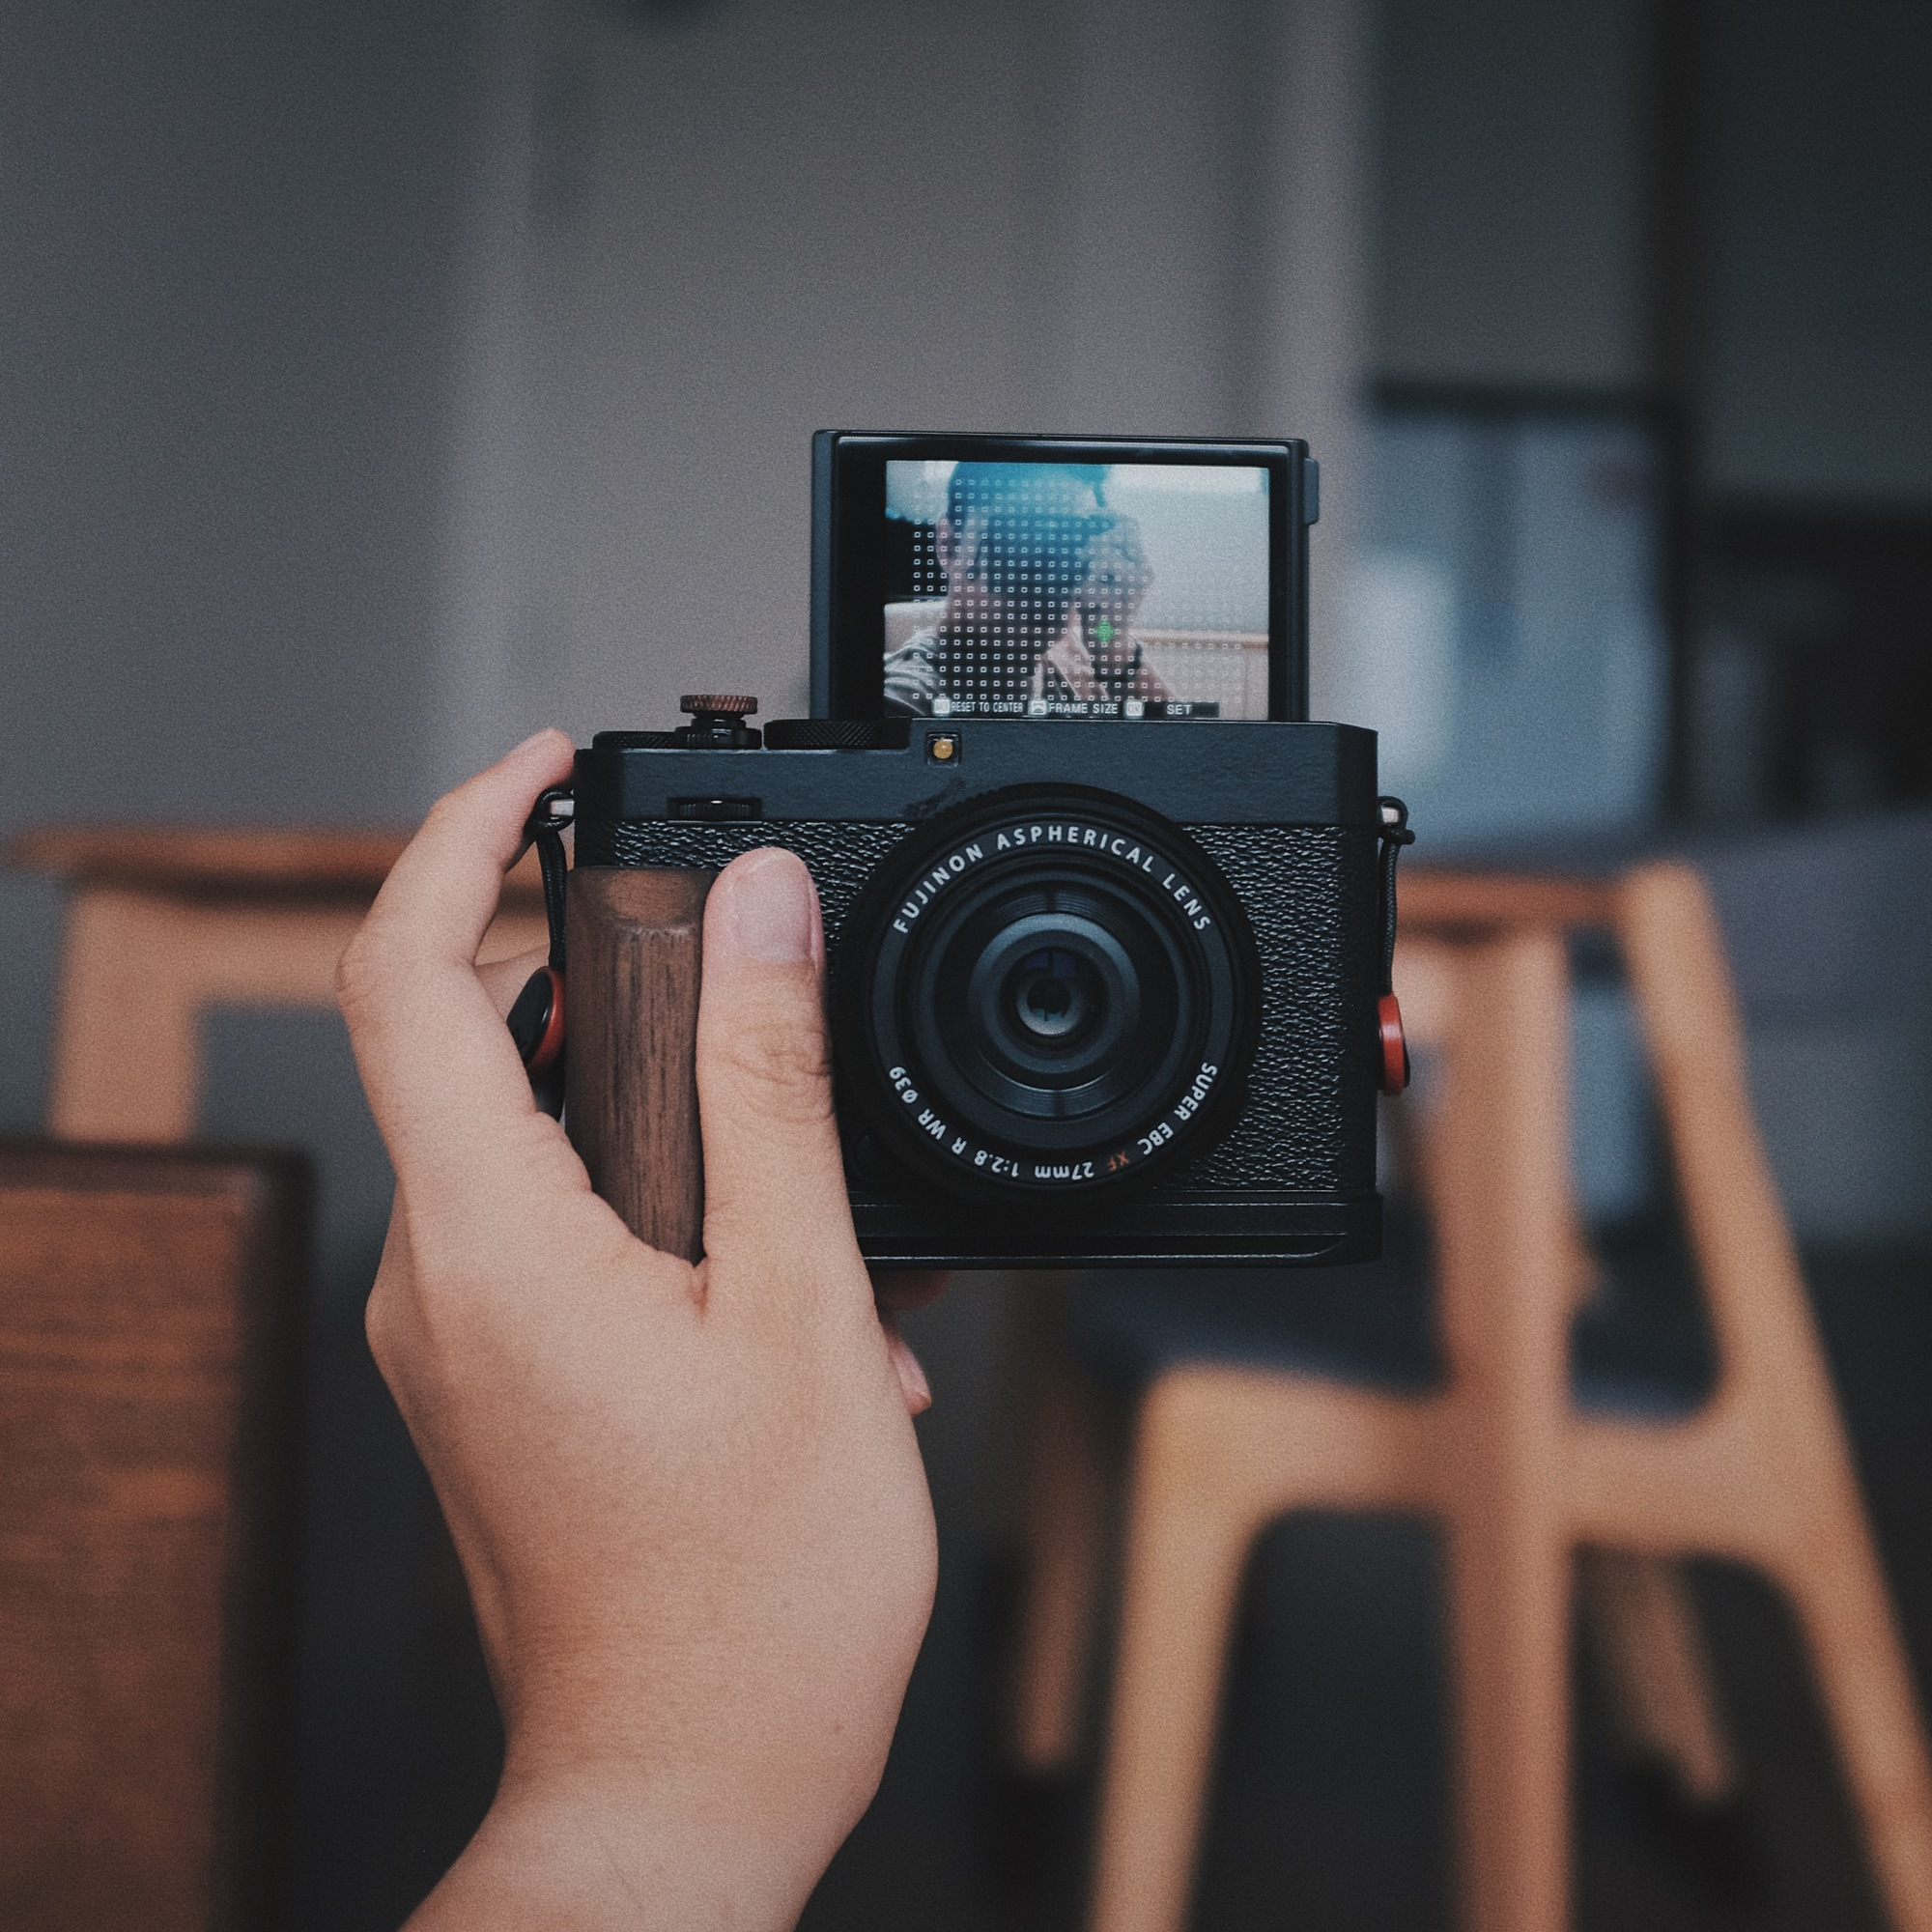
\includegraphics[width=\linewidth]{\envfinaldir/coverpic-prod.jpg}\par
            % \vskip 30pt
            \vfill

            \normalsize\rmfamily\scshape
            \copyright{} The Web Digest Project \hfill\large \envdatestr
        \end{center}
    \end{titlepage}
    % \restoregeometry
}
\newcommand{\simplehref}[1]{%
    \textcolor{blue!80!green}{\href{#1}{#1}}%
}
\renewcommand{\contentsname}{\center\Huge\sffamily\bfseries Contents\par\vskip 20pt}
\newcounter{ipartcounter}
\setcounter{ipartcounter}{0}
\newcommand{\ipart}[1]{
    % \vskip 20pt
    \clearpage
    \stepcounter{ipartcounter}
    \phantomsection
    \addcontentsline{toc}{chapter}{#1}
    % \begin{center}
    %     \Huge
    %     \sffamily\bfseries
    %     #1
    % \end{center}
    % \vskip 20pt plus 7pt
}
\newcounter{ichaptercounter}
\setcounter{ichaptercounter}{0}
\newcommand{\ichapter}[1]{
    % \vskip 20pt
    \clearpage
    \stepcounter{ichaptercounter}
    \phantomsection
    \addcontentsline{toc}{section}{\numberline{\arabic{ichaptercounter}}#1}
    \begin{center}
        \Huge
        \sffamily\bfseries
        #1
    \end{center}
    \vskip 20pt plus 7pt
}
\newcommand{\entrytitlefont}[1]{\subsection*{\raggedright\Large\sffamily\bfseries#1}}
\newcommand{\entryitemGeneric}[2]{
    % argv: title, url
    \parbox{\linewidth}{
        \entrytitlefont{#1}\par\vskip 5pt
        \footnotesize\ttfamily\mdseries
        \simplehref{#2}
    }\vskip 11pt plus 11pt minus 1pt
}
\newcommand{\entryitemGithub}[3]{
    % argv: title, url, desc
    \parbox{\linewidth}{
        \entrytitlefont{#1}\par\vskip 5pt
        \footnotesize\ttfamily\mdseries
        \simplehref{#2}\par\vskip 5pt
        \small\rmfamily\mdseries#3
    }\vskip 11pt plus 11pt minus 1pt
}
\newcommand{\entryitemAp}[3]{
    % argv: title, url, desc
    \parbox{\linewidth}{
        \entrytitlefont{#1}\par\vskip 5pt
        \footnotesize\ttfamily\mdseries
        \simplehref{#2}\par\vskip 5pt
        \small\rmfamily\mdseries#3
    }\vskip 11pt plus 11pt minus 1pt
}
\newcommand{\entryitemHackernews}[3]{
    % argv: title, hnurl, rawurl
    % \parbox{\linewidth}{
    %     \entrytitlefont{#1}\par\vskip 5pt
    %     \footnotesize\ttfamily\mdseries
    %     \simplehref{#3}\par
    %     \textcolor{black!50}{\href{#2}{#2}}
    % }\vskip 11pt plus 11pt minus 1pt
    \begin{minipage}{\linewidth}
            \entrytitlefont{#1}\par\vskip 5pt
            \footnotesize\ttfamily\mdseries
            \simplehref{#3}\par
            \textcolor{black!50}{\href{#2}{#2}}
    \end{minipage}\par\vskip 11pt plus 11pt minus 1pt
}







\begin{document}

\makeheader

\tableofcontents\clearpage




\ipart{Developers}
\ichapter{Hacker News}
\entryitemTwoLinks{How Palantir is mapping the nation's data}{https://news.ycombinator.com/item?id=45215984}{https://theconversation.com/when-the-government-can-see-everything-how-one-company-palantir-is-mapping-the-nations-data-263178}

\entryitemTwoLinks{Nano Banana image examples}{https://news.ycombinator.com/item?id=45215869}{https://github.com/PicoTrex/Awesome-Nano-Banana-images/blob/main/README\_en.md}

\entryitemTwoLinks{Claude's memory architecture is the opposite of ChatGPT's}{https://news.ycombinator.com/item?id=45214908}{https://www.shloked.com/writing/claude-memory}

\entryitemTwoLinks{Top model scores may be skewed by Git history leaks in SWE-bench}{https://news.ycombinator.com/item?id=45214670}{https://github.com/SWE-bench/SWE-bench/issues/465}

\entryitemTwoLinks{Bulletproof host Stark Industries evades EU sanctions}{https://news.ycombinator.com/item?id=45214164}{https://krebsonsecurity.com/2025/09/bulletproof-host-stark-industries-evades-eu-sanctions/}

\entryitemTwoLinks{Native ACME support comes to Nginx}{https://news.ycombinator.com/item?id=45214023}{https://letsencrypt.org/2025/09/11/native-acme-for-nginx}

\entryitemTwoLinks{'Robber bees' invade apiarist's shop in attempted honey heist}{https://news.ycombinator.com/item?id=45213732}{https://www.cbc.ca/news/canada/british-columbia/robber-bees-terrace-bc-apiary-1.7627532}

\entryitemTwoLinks{Spiral}{https://news.ycombinator.com/item?id=45212960}{https://spiraldb.com/post/announcing-spiral}

\entryitemTwoLinks{The US is now the largest investor in commercial spyware}{https://news.ycombinator.com/item?id=45212370}{https://arstechnica.com/security/2025/09/the-us-is-now-the-largest-investor-in-commercial-spyware/}

\entryitemTwoLinks{Conway's Game of Life, but musical}{https://news.ycombinator.com/item?id=45211868}{https://www.hudsong.dev/digital-darwin}

\entryitemTwoLinks{CRISPR offers new hope for treating diabetes}{https://news.ycombinator.com/item?id=45211596}{https://www.wired.com/story/no-more-injections-crispr-offers-new-hope-for-treating-diabetes/}

\entryitemTwoLinks{From burner phones to decks of cards: NYC teens adjusting to the smartphone ban}{https://news.ycombinator.com/item?id=45211527}{https://gothamist.com/news/from-burner-phones-to-decks-of-cards-nyc-teens-are-adjusting-to-the-smartphone-ban}

\entryitemTwoLinks{An engineering history of the Manhattan Project}{https://news.ycombinator.com/item?id=45211127}{https://www.construction-physics.com/p/an-engineering-history-of-the-manhattan}

\entryitemTwoLinks{GrapheneOS and forensic extraction of data (2024)}{https://news.ycombinator.com/item?id=45210910}{https://discuss.grapheneos.org/d/13107-grapheneos-and-forensic-extraction-of-data}

\entryitemTwoLinks{Ireland will not participate in Eurovision if Israel takes part}{https://news.ycombinator.com/item?id=45210867}{https://www.rte.ie/entertainment/2025/0911/1532957-rte-eurovision/}

\entryitemTwoLinks{Behind the scenes of Bun Install}{https://news.ycombinator.com/item?id=45210850}{https://bun.com/blog/behind-the-scenes-of-bun-install}

\entryitemTwoLinks{The rise of async AI programming}{https://news.ycombinator.com/item?id=45210693}{https://www.braintrust.dev/blog/async-programming}

\entryitemTwoLinks{Gregg Kellogg has died}{https://news.ycombinator.com/item?id=45210564}{https://lists.w3.org/Archives/Public/public-json-ld-wg/2025Sep/0012.html}

\entryitemTwoLinks{AirPods live translation blocked for EU users with EU Apple accounts}{https://news.ycombinator.com/item?id=45210428}{https://www.macrumors.com/2025/09/11/airpods-live-translation-eu-restricted/}

\entryitemTwoLinks{Center for the Alignment of AI Alignment Centers}{https://news.ycombinator.com/item?id=45210399}{https://alignmentalignment.ai}\ichapter{Phoronix}
\entryitemGeneric{\hskip 0pt{}Fedora 43 Beta Being Released Next Week}{https://www.phoronix.com/news/Fedora-43-Beta-Next-Week}

\entryitemGeneric{\hskip 0pt{}Linux 6.18 Will Further Complicate Non-GPL Out-Of-Tree File-Systems}{https://www.phoronix.com/news/Linux-6.18-write-cache-pages}

\entryitemGeneric{\hskip 0pt{}Apache Software Foundation Unveils Its Branding Overhaul With New Logo \& "The ASF" Name}{https://www.phoronix.com/news/New-Apache-Software-Logo}

\entryitemGeneric{\hskip 0pt{}Linux Patched For New "VMSCAPE" Vulnerability Affecting Intel \& AMD CPUs}{https://www.phoronix.com/news/Linux-VMSCAPE}

\entryitemGeneric{\hskip 0pt{}CUPS 2.4.13 Print Server Released With "Important" Security Fix}{https://www.phoronix.com/news/CUPS-2.4.13-Released}

\entryitemGeneric{\hskip 0pt{}AMD EPYC 9575F CPUs For GPU/AI Servers Show Leading Performance In Benchmarks}{https://www.phoronix.com/review/amd-epyc-9575f-ai-server}

\entryitemGeneric{\hskip 0pt{}PipeWire 1.4.8 Improves Compatibility With Apple Home Pod Mini Speakers}{https://www.phoronix.com/news/PipeWire-1.4.8-Released}

\entryitemGeneric{\hskip 0pt{}GCC Rust Compiler Continues Quest To Compile The Linux Kernel Crate}{https://www.phoronix.com/news/gccrs-August-2025}

\entryitemGeneric{\hskip 0pt{}Firefox Finally Introducing Matroska / MKV Playback Support}{https://www.phoronix.com/news/Firefox-Nightly-Matroska-MKV}


\ipart{Developers~~~~(zh-Hans)}
\ichapter{Solidot}
\entryitemGeneric{\hskip 0pt{}NASA 禁止中国公民参与其太空项目}{https://www.solidot.org/story?sid=82287}

\entryitemGeneric{\hskip 0pt{}为什么 Netflix 难以制作出高质量电影}{https://www.solidot.org/story?sid=82286}

\entryitemGeneric{\hskip 0pt{}引力波证实霍金黑洞面积定理}{https://www.solidot.org/story?sid=82285}

\entryitemGeneric{\hskip 0pt{}法国配音演员指控《古墓丽影 4-6 重制版》使用 AI 合成其声音}{https://www.solidot.org/story?sid=82284}

\entryitemGeneric{\hskip 0pt{}小红书被要求限期整改}{https://www.solidot.org/story?sid=82283}

\entryitemGeneric{\hskip 0pt{}甲骨文股价飙升,Larry Ellison 成为新首富}{https://www.solidot.org/story?sid=82282}

\entryitemGeneric{\hskip 0pt{}研究发现爱喝啤酒的人对蚊子有高吸引力}{https://www.solidot.org/story?sid=82281}

\entryitemGeneric{\hskip 0pt{}NASA 称毅力号漫游车在火星发现潜在生物特征}{https://www.solidot.org/story?sid=82280}

\entryitemGeneric{\hskip 0pt{}疫情期间使用的一次性口罩留下了化学定时炸弹}{https://www.solidot.org/story?sid=82279}

\entryitemGeneric{\hskip 0pt{}婴儿的哭泣声会让人的身体发热}{https://www.solidot.org/story?sid=82278}

\entryitemGeneric{\hskip 0pt{}Windows 10 拒绝消失}{https://www.solidot.org/story?sid=82277}

\entryitemGeneric{\hskip 0pt{}更温暖的气候可能会增加添加糖摄入量}{https://www.solidot.org/story?sid=82276}

\entryitemGeneric{\hskip 0pt{}海洋暖化危及食物网关键物种原绿球藻}{https://www.solidot.org/story?sid=82275}

\entryitemGeneric{\hskip 0pt{}任天堂获得召唤物并让召唤物战斗的美国专利}{https://www.solidot.org/story?sid=82274}

\entryitemGeneric{\hskip 0pt{}天文学家在棕矮星发现硅烷}{https://www.solidot.org/story?sid=82273}

\entryitemGeneric{\hskip 0pt{}早期宇宙磁场强度与人脑神经元相当}{https://www.solidot.org/story?sid=82272}

\entryitemGeneric{\hskip 0pt{}美国股市不再有超额收益}{https://www.solidot.org/story?sid=82271}

\entryitemGeneric{\hskip 0pt{}巴基斯坦的大规模监控系统}{https://www.solidot.org/story?sid=82270}

\entryitemGeneric{\hskip 0pt{}微软强制执行重返办公室政策}{https://www.solidot.org/story?sid=82269}

\entryitemGeneric{\hskip 0pt{}苹果发布 iPhone 17 系列手机,推出超薄型号 iPhone Air}{https://www.solidot.org/story?sid=82268}\ichapter{V2EX}
\entryitemGeneric{\hskip 0pt{}[问与答] 运营商推荐}{https://www.v2ex.com/t/1158675}

\entryitemGeneric{\hskip 0pt{}[职场话题] 最近一线城市 web 前端好找工作吗}{https://www.v2ex.com/t/1158673}

\entryitemGeneric{\hskip 0pt{}[程序员] 求瑞幸 库迪 蜜雪 甜啦 肯德基 等等货源接口}{https://www.v2ex.com/t/1158672}

\entryitemGeneric{\hskip 0pt{}[Apple] 请教一下外版的苹果设备该怎么买 apple care}{https://www.v2ex.com/t/1158671}

\entryitemGeneric{\hskip 0pt{}[程序员] 吐槽一下某些网站的前端设计,无限滚动搭配页脚}{https://www.v2ex.com/t/1158670}

\entryitemGeneric{\hskip 0pt{}[iPhone] 外版 iPhone17 回国新方案:卡贴机、苹果皮重现江湖}{https://www.v2ex.com/t/1158669}

\entryitemGeneric{\hskip 0pt{}[问与答] 工行 visa 卡,有必要开通这个外币自动还款吗?}{https://www.v2ex.com/t/1158668}

\entryitemGeneric{\hskip 0pt{}[求职] [社招] 影石 insta360, 34 个急招岗位,技术/非技术}{https://www.v2ex.com/t/1158667}

\entryitemGeneric{\hskip 0pt{}[Apple] iPhone 17 哪个地区的是满血版}{https://www.v2ex.com/t/1158666}

\entryitemGeneric{\hskip 0pt{}[问与答] 创意方案:远端如何统计不联网的电视机开关时间?}{https://www.v2ex.com/t/1158665}

\entryitemGeneric{\hskip 0pt{}[职场话题] 请教各位,在这样的公司做开发有没有法律风险}{https://www.v2ex.com/t/1158663}

\entryitemGeneric{\hskip 0pt{}[macOS] 小番喜-PomoJoy, 又一款番茄时钟 APP 加入了内卷大军}{https://www.v2ex.com/t/1158662}

\entryitemGeneric{\hskip 0pt{}[分享创造] 分享一个刚做完的 AI 图像处理工具,技术栈挺有意思的}{https://www.v2ex.com/t/1158661}

\entryitemGeneric{\hskip 0pt{}[NAS] 写了个家庭 AIO 服务器搭建教程}{https://www.v2ex.com/t/1158660}

\entryitemGeneric{\hskip 0pt{}[生活] 今天得知大学同学进了字节}{https://www.v2ex.com/t/1158658}

\entryitemGeneric{\hskip 0pt{}[iPhone] 买港版 iPhone 的方法}{https://www.v2ex.com/t/1158657}

\entryitemGeneric{\hskip 0pt{}[职场话题] 跳槽收到 offer 后的一些迷茫,求建议}{https://www.v2ex.com/t/1158656}

\entryitemGeneric{\hskip 0pt{}[生活] 兄弟们 跪求 有用的灭小黄蚂蚁的药和方式}{https://www.v2ex.com/t/1158655}

\entryitemGeneric{\hskip 0pt{}[远程工作] 远程招募: PHP 开发 ,需求多名,薪资面议}{https://www.v2ex.com/t/1158654}

\entryitemGeneric{\hskip 0pt{}[iPhone] 天猫官旗以旧换新购买 iPhone 17,补贴 1300,天猫回收有坑不?}{https://www.v2ex.com/t/1158653}

\entryitemGeneric{\hskip 0pt{}[问与答] 两台 android 手机 如何免费 实现 远程控制?}{https://www.v2ex.com/t/1158651}

\entryitemGeneric{\hskip 0pt{}[分享创造] 以键盘为核心: SideCalendar 三层键盘交互的设计思考}{https://www.v2ex.com/t/1158650}

\entryitemGeneric{\hskip 0pt{}[虚拟现实] Quest3 看片}{https://www.v2ex.com/t/1158649}

\entryitemGeneric{\hskip 0pt{}[分享创造] 最近写了一个在浏览器中运行的 PDF 工具集}{https://www.v2ex.com/t/1158648}

\entryitemGeneric{\hskip 0pt{}[问与答] 有没有发现 Garmin Connect 强制跳转到国区了。}{https://www.v2ex.com/t/1158647}

\entryitemGeneric{\hskip 0pt{}[问与答] 谁有商业派安盈账户,帮我转一笔小款}{https://www.v2ex.com/t/1158646}

\entryitemGeneric{\hskip 0pt{}[香港] 求助,香港东亚银行账户被冻结怎么办?}{https://www.v2ex.com/t/1158645}

\entryitemGeneric{\hskip 0pt{}[程序员] 2025 第四季度了,移动端开发你会选择 flutter 还是 react native?}{https://www.v2ex.com/t/1158644}

\entryitemGeneric{\hskip 0pt{}[问与答] clash meta 无法仅允许已选择的应用 无法生效}{https://www.v2ex.com/t/1158643}

\entryitemGeneric{\hskip 0pt{}[问与答] 新买的 265k 和技嘉小雕 z890m 通过核显连显示器怎么都点不亮}{https://www.v2ex.com/t/1158642}

\entryitemGeneric{\hskip 0pt{}[React] React 19 下有什么方便点的组件? Arco Design 用起来还是有些问题}{https://www.v2ex.com/t/1158641}

\entryitemGeneric{\hskip 0pt{}[iPhone] 美区 Paypal 冻结导致 Appstore 出现死循环}{https://www.v2ex.com/t/1158640}

\entryitemGeneric{\hskip 0pt{}[职场话题] 跟律所某律师主任合作 5 年左右的经历}{https://www.v2ex.com/t/1158639}

\entryitemGeneric{\hskip 0pt{}[问与答] [杭州] [12-24k] [AI SaaS] 运维工程师}{https://www.v2ex.com/t/1158638}

\entryitemGeneric{\hskip 0pt{}[以太坊] 区块链 PHP 。区块链产品经理 ,五年以上经验}{https://www.v2ex.com/t/1158637}

\entryitemGeneric{\hskip 0pt{}[iPhone] 附近几个地区的 iPhone 价格咋样?}{https://www.v2ex.com/t/1158635}

\entryitemGeneric{\hskip 0pt{}[问与答] 四川电信 iMessage 今日突然大面积恢复激活}{https://www.v2ex.com/t/1158634}

\entryitemGeneric{\hskip 0pt{}[全球工单系统] 原来微信会吞消息,不是吞一条,而是吞一半}{https://www.v2ex.com/t/1158633}

\entryitemGeneric{\hskip 0pt{}[Apple] 港版 iPhone 只能用一张实体卡了求大家推荐一张主卡}{https://www.v2ex.com/t/1158632}

\entryitemGeneric{\hskip 0pt{}[生活] 才发现银行卡被限额 5000}{https://www.v2ex.com/t/1158631}

\entryitemGeneric{\hskip 0pt{}[Apple] 去年为了 AI 特地去日本买了 16}{https://www.v2ex.com/t/1158629}

\entryitemGeneric{\hskip 0pt{}[MySQL] count 的语句优化问题}{https://www.v2ex.com/t/1158628}

\entryitemGeneric{\hskip 0pt{}[程序员] 有没有好用的数据库连接工具推荐一下}{https://www.v2ex.com/t/1158627}

\entryitemGeneric{\hskip 0pt{}[macOS] macos 删除文件后空间怎么释放出来}{https://www.v2ex.com/t/1158625}

\entryitemGeneric{\hskip 0pt{}[Claude] Claude Code 拼车(Max 版本)}{https://www.v2ex.com/t/1158624}

\entryitemGeneric{\hskip 0pt{}[云计算] 我有 80 万张图片在阿里云,如何存比较合适?}{https://www.v2ex.com/t/1158623}

\entryitemGeneric{\hskip 0pt{}[职场话题] 离开职场两年,我终于学会与迷茫共处}{https://www.v2ex.com/t/1158622}

\entryitemGeneric{\hskip 0pt{}[Web3] Nwb***8899 这个钱包每 10 分钟小额买入一次 \$v2ex 且不是手续费很高?}{https://www.v2ex.com/t/1158621}

\entryitemGeneric{\hskip 0pt{}[问与答] 有辞职的老铁吗?企业年金怎么处理?}{https://www.v2ex.com/t/1158620}

\entryitemGeneric{\hskip 0pt{}[创业组队] 星巴克代下渠道求认识|我能做下单/风控/对账一条龙}{https://www.v2ex.com/t/1158619}


\ipart{Generic News}







\clearpage
\leavevmode\vfill
\footnotesize

Copyright \copyright{} 2023-2025 Neruthes and other contributors.

This document is published with CC BY-NC-ND 4.0 license.

The entries listed in this newsletter may be copyrighted by their respective creators.

This newsletter is generated by the Web Digest project.

The newsletters are also delivered via Telegram channel \CJKunderline{\href{https://t.me/webdigestchannel}{https://t.me/webdigestchannel}}.\\
RSS feed is available at \CJKunderline{\href{https://webdigest.pages.dev/rss.xml}{https://webdigest.pages.dev/rss.xml}}.

This newsletter is available in PDF at
\CJKunderline{\href{https://webdigest.pages.dev/}{https://webdigest.pages.dev/}}.

The source code being used to generate this newsletter is available at\\
\CJKunderline{\href{https://github.com/neruthes/webdigest}{https://github.com/neruthes/webdigest}}.

This newsletter is also available in
\CJKunderline{\href{http://webdigest.pages.dev/readhtml/\envyear/WebDigest-20250912.html}{HTML}} and
\CJKunderline{\href{https://github.com/neruthes/webdigest/blob/master/markdown/\envyear/WebDigest-20250912.md}{Markdown}}.


\coverpic{https://unsplash.com/photos/modern-building-with-red-accent-against-blue-sky-jLw5cNBOz3s}{Liu water}


\end{document}
